% THIS IS SIGPROC-SP.TEX - VERSION 3.1
% WORKS WITH V3.2SP OF ACM_PROC_ARTICLE-SP.CLS
% APRIL 2009
%
% It is an example file showing how to use the 'acm_proc_article-sp.cls' V3.2SP
% LaTeX2e document class file for Conference Proceedings submissions.
% ----------------------------------------------------------------------------------------------------------------
% This .tex file (and associated .cls V3.2SP) *DOES NOT* produce:
%       1) The Permission Statement
%       2) The Conference (location) Info information
%       3) The Copyright Line with ACM data
%       4) Page numbering
% ---------------------------------------------------------------------------------------------------------------
% It is an example which *does* use the .bib file (from which the .bbl file
% is produced).
% REMEMBER HOWEVER: After having produced the .bbl file,
% and prior to final submission,
% you need to 'insert'  your .bbl file into your source .tex file so as to provide
% ONE 'self-contained' source file.
%
% Questions regarding SIGS should be sent to
% Adrienne Griscti ---> griscti@acm.org
%
% Questions/suggestions regarding the guidelines, .tex and .cls files, etc. to
% Gerald Murray ---> murray@hq.acm.org
%
% For tracking purposes - this is V3.1SP - APRIL 2009

%\documentclass{acm_proc_article-sp}

\documentclass{sig-alternate}
\usepackage[numbers, sort, compress]{natbib}
\usepackage{xspace}
\usepackage{color}
\usepackage{url}
%\usepackage{hyphenation}
\hyphenation{Map-Reduce}

\newif\ifdraft
\drafttrue

\ifdraft
\newcommand{\terminology}[1]{ {\textcolor{red} {(Terminology used: \textbf{#1}) }}}
\newcommand{\jhanote}[1]{ {\textcolor{red} { ***shantenu: #1 }}}
\newcommand{\alnote}[1]{ {\textcolor{blue} { ***andreL: #1 }}}
\newcommand{\pnote}[1]{ {\textcolor{magenta} { ***pradeep: #1 }}}
\newcommand{\note}[1]{ {\textcolor{brown} { ***Note: #1 }}}
\else
\newcommand{\terminology}[1]{}
\newcommand{\alnote}[1]{}
\newcommand{\pnote}[1]{}
\newcommand{\jhanote}[1]{}
\newcommand{\note}[1]{}
\fi



\newcommand{\pilot}{Pilot\xspace}
\newcommand{\pilots}{Pilots\xspace}
\newcommand{\pilotjob}{Pilot-Job\xspace}
\newcommand{\pilotjobs}{Pilot-Jobs\xspace}
\newcommand{\pilotmapreduce}{Pilot-MapReduce\xspace}
\newcommand{\computeunit}{Compute Unit\xspace}
\newcommand{\computeunits}{Compute Units\xspace}
\newcommand{\cu}{CU\xspace}
\newcommand{\cus}{CUs\xspace}
\newcommand{\cs}{Compute Service\xspace}
\newcommand{\css}{Compute Services\xspace}
\newcommand{\pcs}{Pilot Compute Service\xspace}
\newcommand{\dataunit}{Data Unit\xspace}
\newcommand{\dataunits}{Data Unit\xspace}
\newcommand{\du}{DU\xspace}
\newcommand{\dus}{DUs\xspace}
\newcommand{\pilotdata}{Pilot-Data\xspace}
\newcommand{\pd}{PD\xspace}
\newcommand{\pds}{Pilot Data Service\xspace}
\newcommand{\pdss}{Pilot Data Services\xspace}
\newcommand{\su}{SU\xspace}
\newcommand{\sus}{SUs\xspace}
\newcommand{\schedulableunit}{Schedulable Unit\xspace}
\newcommand{\schedulableunits}{Schedulable Units\xspace}
\begin{document}

\title{An extensible Pilot-based MapReduce Implementation}

%
% You need the command \numberofauthors to handle the 'placement
% and alignment' of the authors beneath the title.
%
% For aesthetic reasons, we recommend 'three authors at a time'
% i.e. three 'name/affiliation blocks' be placed beneath the title.
%
% NOTE: You are NOT restricted in how many 'rows' of
% "name/affiliations" may appear. We just ask that you restrict
% the number of 'columns' to three.
%
% Because of the available 'opening page real-estate'
% we ask you to refrain from putting more than six authors
% (two rows with three columns) beneath the article title.
% More than six makes the first-page appear very cluttered indeed.
%
% Use the \alignauthor commands to handle the names
% and affiliations for an 'aesthetic maximum' of six authors.
% Add names, affiliations, addresses for
% the seventh etc. author(s) as the argument for the
% \additionalauthors command.
% These 'additional authors' will be output/set for you
% without further effort on your part as the last section in
% the body of your article BEFORE References or any Appendices.

\numberofauthors{3} %  in this sample file, there are a *total*
% of EIGHT authors. SIX appear on the 'first-page' (for formatting
% reasons) and the remaining two appear in the \additionalauthors section.
%
\author{
% You can go ahead and credit any number of authors here,
% e.g. one 'row of three' or two rows (consisting of one row of three
% and a second row of one, two or three).
%
% The command \alignauthor (no curly braces needed) should
% precede each author name, affiliation/snail-mail address and
% e-mail address. Additionally, tag each line of
% affiliation/address with \affaddr, and tag the
% e-mail address with \email.
%
\alignauthor Pradeep Kumar Mantha\\
       \affaddr{Center for Computation and Technology}\\
       \affaddr{Louisiana State University}\\
       \affaddr{216 Johnston}\\
       \affaddr{Baton Rouge, LA}
       \email{pmanth2@cct.lsu.edu}
\alignauthor Andre Luckow\\
       \affaddr{Center for Computation and Technology}\\
       \affaddr{Louisiana State University}\\
       \affaddr{216 Johnston}\\
       \affaddr{Baton Rouge, LA}
       \email{aluckow@cct.lsu.edu} 
\alignauthor Shantenu Jha\titlenote{Author for correspondence}\\
      \affaddr{Center for Autonomic Computing}\\
     \affaddr{Rutgers University}\\
      \affaddr{94 Brett Road}\\
      \affaddr{Piscataway, NJ}
     \email{shantenu.jha@rutgers.edu}
}
% There's nothing stopping you putting the seventh, eighth, etc.
% author on the opening page (as the 'third row') but we ask,
% for aesthetic reasons that you place these 'additional authors'
% in the \additional authors block, viz.
% \additionalauthors{Additional authors: John Smith (The Th{\o}rv{\"a}ld Group,
% email: {\texttt{jsmith@affiliation.org}}) and Julius P.~Kumquat
% (The Kumquat Consortium, email: {\texttt{jpkumquat@consortium.net}}).}
\date{30 July 1999}
% Just remember to make sure that the TOTAL number of authors
% is the number that will appear on the first page PLUS the
% number that will appear in the \additionalauthors section.

\maketitle
\begin{abstract}
In recent years, there has been a large increase in the size of computational
data which is widely distributed across different geographic locations. Timing and
cost-effective processing of these large-distributed datasets on distributed
computational resources requires effective management of data and compute
resources. Pilot-Jobs are successful in uptaking the distributed
infrastructures by compute intensive applications, but still there is a
necessity of an abstraction for data intensive applications to provide
coupling between data and compute units through a set of relationships.
Pilot-Data provides an abstraction for expressing and managing relationships
between data and/or compute units. The coupling of Pilot abstractions,
Pilot-Job and Pilot-Data, through SAGA Pilot API implementation, provides
flexibility to specify the relationship between compute and data units and
thus effective management of compute and data units across distributed
infrastructures. MapReduce is an effective programming model for processing
large distributed datasets. However, processing widely-distributed data sets
using traditional MapReduce setup configurations limits concurrent usage of
distributed infrastructure and depending on the type of workload aggregation,
overheads like huge data transfers or additional computation to combine
results are involved [weissmanns]. Most MapReduce implementations however,
tied to specific infrastructure. In this paper, we describe the design and
implementation of Pilot API based SAGA MapReduce (PMR), which is 
infrastructure
independent and extensible to multiple clusters. We validate and characterize
PMR by benchmarking it with Hadoop MapReduce using canonical word count
application. We present a PMR workflow to post-process data produced by deep
sequencing machines at widely-distributed geographic locations. The workflow
takes the output of the sequencing machines, performs short-read mapping using
BWA aligner, and removes duplicate reads. Our experiments show that it
provided a significantly improved throughput as it scaled to multiple
clusters, over traditionally distributed MapReduce~\cite{weissman-mr-11}.
\end{abstract}

% A category with the (minimum) three required fields
\category{D.1.2}{Software}{MapReduce}
%A category including the fourth, optional field follows...
\category{J.3}{Computer Applications}{Bioinformatics, Mapping}

% \terms{Design, Experimentation, Performance}

\keywords{Pilot-Jobs, Pilot-Data, Data-Intensive, MapReduce, Genome Sequence
Alignment, BWA, Human Genome, MapReduce, Distributed Computing, Simple API for
Grid Applications (SAGA)}% NOT required for Proceedings

\section{Introduction}

%General Motivation
There are various challenges associated with data at extreme scales: which
have become a critical factor in many sciences disciplines, e.\,g.\ in the
areas of fusion energy (ITER), bioinformatics (metagenomics), climate (Earth
System Grid), and astronomy
(LSST)~\cite{Berriman:2011:AAS:2039359.2047483,Jha:2011fk}. The volumes of
data produced by these scientific applications are increasing rapidly driven
by advancing technologies (e.\,g.\ increasing compute capacity and higher
resolution sensors) and decreasing costs for computation, data acquisition and
storage~\cite{hey2009}. The number of scientific applications that either
currently utilize, or need to utilize large volumes of potentially distributed
data is immense. The challenges faced by these applications are
interoperability, efficiently managing compute tasks, and moving data to the
scheduled compute location, which is inevitable in case of programming models
like MapReduce.

%Intro to MapReduce
Processing large volumes of data is a challenging tasks. MapReduce is an
effective programming model for addressing this challenge.
MapReduce~\cite{Dean:2004:MSD:1251254.1251264} as originally developed by
Google aims to address the big data problem by providing an easy-to-use
abstraction for parallel data processing. The most prominent framework for 
doing MapReduce computations is Apache Hadoop~\cite{hadoop}. The main 
limitations of current MR implementations are: (i) They lack a modular 
architecture, (ii) are tied to specific infrastructure, e.\,g.\ Hadoop relies 
on the Hadoop File System (HDFS), and  (iii) do not provide efficient support 
for dynamic and distributed data.

% In particular when the source
% data and computing platform distributed widely, the most efficient
% architecture for processing data over the entire data set becomes non-trivial.


%Why pilot abstractions
Pilot-Jobs have been notable in their ability to manage large numbers of
compute units across multiple high performance clusters, providing decoupling
application-level scheduling and system-level resource management. But, there
is also a need of an abstraction to liberate applications/users from
challenging requirement of moving data to the scheduled compute location to
execute it successfully. Pilot-Data provides an abstraction for expressing and
managing relationships between data units and/or compute units. The coupling
of abstractions, Pilot-Jobs and Pilot-Data, provide a complete solution for
data intensive applications to utilize distributed cyber infrastructure
effectively. The Pilot-API is an implementation of P* model, and provides
flexibility to manage compute, data and relationships between them
(affinities)~\cite{pstar-2012}.


In this paper, we \pilotmapreduce -- a new \pilot based MapReduce
implementation. \pilot abstractions enable the clean separation of resource
management and MapReduce application. A critical aspect of MapReduce, is the
management of data/compute localities as well as the management of data
movements, e.\,g.\ between the mapping and the reduction phase. The efficient
support of these capabilities via the \pilot abstractions as well as the
limitations of existing MapReduce implementations motivated this work. We show
how \pilot abstractions are used for managing the map and reduce tasks and
intermediate shuffle data between them.

The key take-aways of this paper are:
\begin{itemize}
	\item MapReduce simplifies the construction of data-parallel applications
	\item Pilot-Abstraction enable the clean separation of resource management concerns and MapReduce.
	\item The Pilot/SAGA-based approach enables a maximum of portability, interoperability and code-reuse.
	\item Hadoop is designed for cluster/local environment, but not for a high degree of distribution.
	\item Future work: dynamic execution
\end{itemize}

In section II we talk about background-- Pilot API, Pilot-Job, Pilot-Data,
saga, SAGA previous implementation of MapReduce, Genome sequencing MapReduce
application. In section III, we discuss how Pilot abstractions, Pilot-Job and
Pilot-Data used to implement the architecture of MapReduce.,. In section IV we
discuss about the experiments.

\section{Related Work}

The MapReduce programming model~\cite{Dean:2004:MSD:1251254.1251264} and the
distributed file system (Google File System
(GFS)~\cite{Ghemawat:2003:GFS:1165389.945450}) it is based on was originally
pioneered by Google. Apache Hadoop~\cite{hadoop} is an open source
implementation of MapReduce. Hadoop also includes an implementation of a
distributed file system -- the Hadoop File System
(HDFS)~\cite{Borthakur:2007fk}. In addition the Hadoop ecosystems includes
several other projects, such as HBase (a system also inspired by Google's
BigTable), Hive, Pig and Zookeeper.

Sector/Sphere~\cite{Gu_Grossman_2009} is a parallel data processing framework
consisting of an distributed file system (Sector) and a data processing engine
(Sphere). In contrast to Hadoop, Sphere is able to execute arbitrary 
user-defined function on a stream of data. Hadoop in contrast operates on top 
of file system chunks.

Twister~\cite{Ekanayake:2010:TRI:1851476.1851593} is a 
MapReduce addressing particularly the requirement for supporting iterative 
MapReduce jobs. Twister allows the flexible composition of applications by 
specifying map and reduce tasks and the data flow between these tasks. 


SAGA-MapReduce~\cite{Sehgal:2011:UAI:1945091.1945329} is a SAGA-based
MapReduce implementation that utilizes the SAGA-API for accessing system-level
features, such as resource management, file management and coordination. The
SAGA-based approach enabled the decoupling of infrastructure and application
concerns enabling the support of a wide-set of distributed infrastructure
(e.\,g,\ grids and clouds). The utilization of Pilot abstractions has several
advantages compared to the SAGA-only approach: (i) compute and data pilots
allow an efficient decoupling of resource allocation and usage, i.\,e.\ the
MapReduce master can efficiently schedule compute units containing mapper and
reduce tasks; (ii) the co-location of data and compute units descriptively
defined and are automatically handled by Pilot framework; This enables the
applications to easily trade-off data transfers and available compute
capacities.

The main limitation of MapReduce and in particular of Hadoop is that it forces
applications into a very rigid model. Hadoop e.\,g.\ is well suited for
running single applications, but very limited in terms of extensibility,
e.\,g.\ it cannot efficiently run an ensemble of MapReduce simulations or
support a pipeline of multiple MapReduce tasks. In this paper we present a 
MapReduce implementation that utilizes \pilot abstractions for de-coupling the MapReduce runtime, application-level scheduling and resource management.

%data flow oriented frameworks


Dryad

Twitter Storm

\section{Pilot Compute and Pilot Data}

Pilot-Jobs support effective distributed resource utilization, and are arguably one of the most widely-used distributed computing abstractions. 

\subsection{Pilot Abstractions for Compute and Data}

The abstraction of a {\emph \pilotjob} generalizes the reoccurring concept of
utilizing a placeholder job as a container for a set of compute tasks;
instances of that placeholder job are commonly referred to as Pilot-Jobs or
pilots. The PJ provides applications (user) level control and management of
the set of allocated resources. Analogous to \pilotjobs, {\emph Pilot-Data}
provides late-binding capabilities for data by separating the allocation of
physical storage and application-level data units~\cite{pstar-2012}.

The Pilot-API exposes the core functionalities of a \pilot framework via a
unified interface providing a common API that can be used across multiple PJ
frameworks. The API provides three core classes: the
\texttt{PilotComputeService} for the management of Pilot-Jobs,
\texttt{PilotDataService} for the management of Pilot-Data and the
\texttt{ComputeDataService} for the management of \texttt{ComputeUnits} (CUs)
and \texttt{DataUnits} (DUs). A CU represents a primary self-containing piece
of work, while a DU represents a logical set for data~\cite{pstar-2012}.

\subsection{BigData: A Pilot-Data Implementation}
\begin{figure}[htbp]
	\centering
		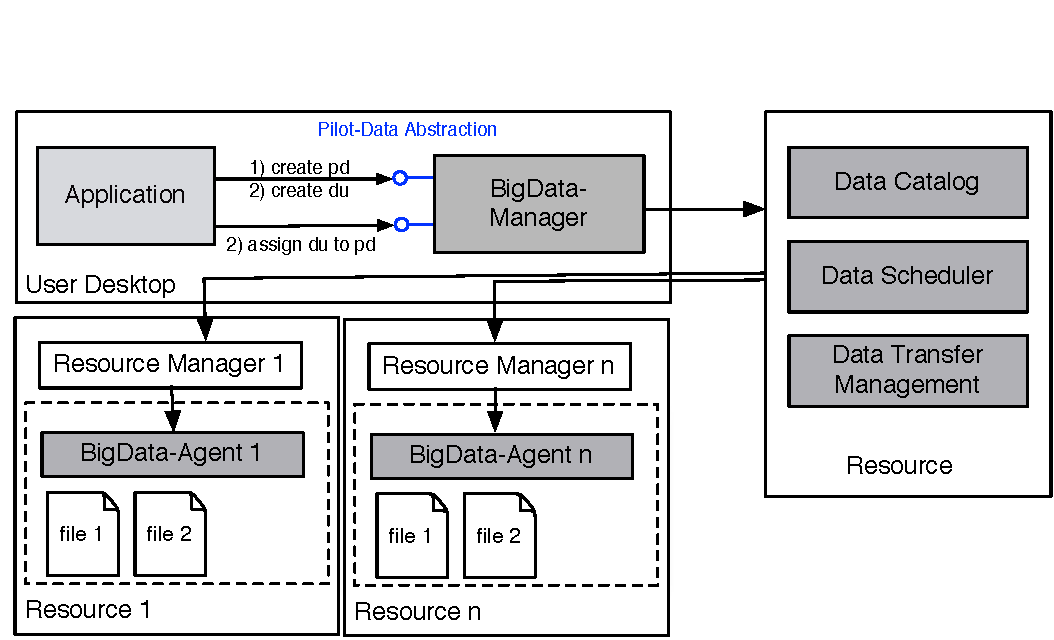
\includegraphics[width=0.47\textwidth]{figures/bigdata.pdf}
	\caption{BigData Architecture and Interactions}
	\label{fig:figures_bigdata}
\end{figure}

{\it BigData (BD)} is an implementation of the Pilot-Data abstraction.
BigData is based on BigJob~\cite{bigjob_web} -- a SAGA-based Pilot-Job
implementation. Figure~\ref{fig:figures_bigdata} gives an overview of the
architecture. The system consists similarly to BigJob of two components: the
BD-Manager and the BD-Agents deployed on the physical resources. The
coordination scheme used is again M/W with some intelligence that is located
de-centrally at the BD-Agent. As communication mechanism the SAGA Advert
Service is used, in a similar push/pull mode as for BJ.

The BD-Manager is responsible for (i) meta-data management, i.\,e.\ it
keeps track of the pilot stores that a pilot data object is associated
with, (ii) for scheduling data movements and data replications (taking
into account the application requirements defined via affinities), and
(iii) for managing data movements activities. For this purpose, it can rely
on external service, e.\,g.\ Globus Online for data transfer management.  
Similar to BigJob, an agent on each resource is used to manage the physical 
storage on a resource.  

A particular critical requirement for data-intensive application, is
the management of affinity between CUs and also between DUs and
DUs. The BD scheduler supports preliminary affinity-aware
scheduling: both BigJob and BigData are tightly integrated to
efficiently support compute- and data-related aspects of dynamic
execution.


\section{Pilot-MapReduce -- A Pilot-based MapReduce Implementation}
\alnote{We should only use PilotMapReduce to refer to our framework - SAGA does not need to be in the name and mentioned all the time}


{\emph \pilotmapreduce} provides a \pilot based implementation of the 
MapReduce programming model decoupling the core MapReduce framework from the 
actual management of the compute, data and network resources. By decoupling 
job scheduling and monitoring from the resource management, \pilotmapreduce 
can efficiently re-use the resource management and late-binding capabilities 
of BigJob and BigData.

\pilotmapreduce exposes an easy-to-use interface which provides the complete
functionality needed by any MapReduce algorithm, while hiding the more complex
functionality, such as chunking of the input, sorting the intermediate
results, managing and coordinating the map \& reduce tasks, etc., these are generically
implemented by the framework.

\alnote{Can we put a code snipped in here somewhere? maybe a separate sub-section}

\pilotmapreduce uses the Pilot-API for managing map and reduce compute and intermediate data.

%Pilot-API is used for managing map and reduce compute units
%and for defining relationships between the intermediate data and reduce tasks
%across distributed infrastructure

\subsection{Compute Management}
The framework relies on the master/worker
coordination model, i.\,e.\ a central MapReduce-Manager is responsible for
coordinating the MapReduce workers, which again are responsible for executing
map and reduce tasks. The MR-Manager utilizes BigJob for executing
mapper and reduce tasks. 

Similarly, Hadoop also utilizes a job and task tracker: the job tracker is the
central manager that dispatches map and reduce tasks to the nodes of the
Hadoop cluster. On each node the task tracker is responsible for executing the
respective tasks. The main limitation of this architecture is the fact that it
intermixes both cluster resource management and application-level task
managements. Thus, it is e.\,g.\ not easily possible to integrate Hadoop with
another resource management tool, e.\,g.\ PBS or Torque. Also, the job tracker
represents a single point of failure and scalability bottleneck

\subsection{Data Management}
\alnote{We haven't introduced the notion of distributed pilot map reduce.}
The efficiency of distributed MapReduce on multiple clusters depends on managing the
intermediate data between them. BigData does not only provides flexibility to manage the
relationship between data and compute units, but also allow {\it parallel} data transfers
between machines and between data units. BigData is particularly used for moving the
intermediate output files of the mapper tasks to the resource where the reduce compute
units are executed. In distributed \pilotmapreduce on m clusters with n reduces distributed
evenly across clusters involve n*(m-1) parallel data transfers to complete the intermediate
data movement.


\pnote{
   comparing data transfer with Hadoop data transfer.
Hadoop-Data transfer - "Separate nodes in a Hadoop cluster still communicate with one another. However, in contrast to more conventional distributed systems where application developers explicitly marshal byte streams from node to node over sockets or through MPI buffers, communication in Hadoop is performed implicitly. Pieces of data can be tagged with key names which inform Hadoop how to send related bits of information to a common destination node. Hadoop internally manages all of the data transfer and cluster topology issues."
Similarly - A group of files is represented by a data unit
mapred.reduce.parallel.copies		The default number of parallel transfers run by reduce during the copy(shuffle) phase.
Concurrent data transfers... allowed..between machines and nodes.}



\subsection{Architecture of Pilot-MapReduce}


%The framework relies on the master/worker
%coordination model, i.\,e.\ a central MapReduce-Manager is responsible for
%coordinating the MapReduce workers, which again are responsible for executing
%map and reduce tasks. The MR-Manager utilizes BigJob for executing
%mapper and reduce tasks, and BigData for managing file transfers.
%BigData is particularly used for moving the intermediary output files of
%the mapper tasks to the resource where the reduce compute units are executed.

%Similarly, Hadoop also utilizes a job and task tracker: the job tracker is the
%central manager that dispatches map and reduce tasks to the nodes of the
%Hadoop cluster. On each node the task tracker is responsible for executing the
%respective tasks. The main limitation of this architecture is the fact that it
%intermixes both cluster resource management and application-level task
%managements. Thus, it is e.\,g.\ not easily possible to integrate Hadoop with
%another resource management tool, e.\,g.\ PBS or Torque. Also, the job tracker
%represents a single point of failure and scalability bottleneck.
Pilot-MapReduce introduces a clean separation of concerns regarding compute and data management. The
pilot abstraction enable the easy acquisition of both compute and storage
resources. The MR manager can focus on orchestrating this resource pool. This architecture can also efficiently support workloads that currently cannot be support well enough by Hadoop, e.\,g.\ iterative applications. Figure~\ref{fig:figures_mapreduce-pilotdata} shows the architecture of the
\pilotmapreduce framework.

\begin{figure}[htbp]
	\centering
	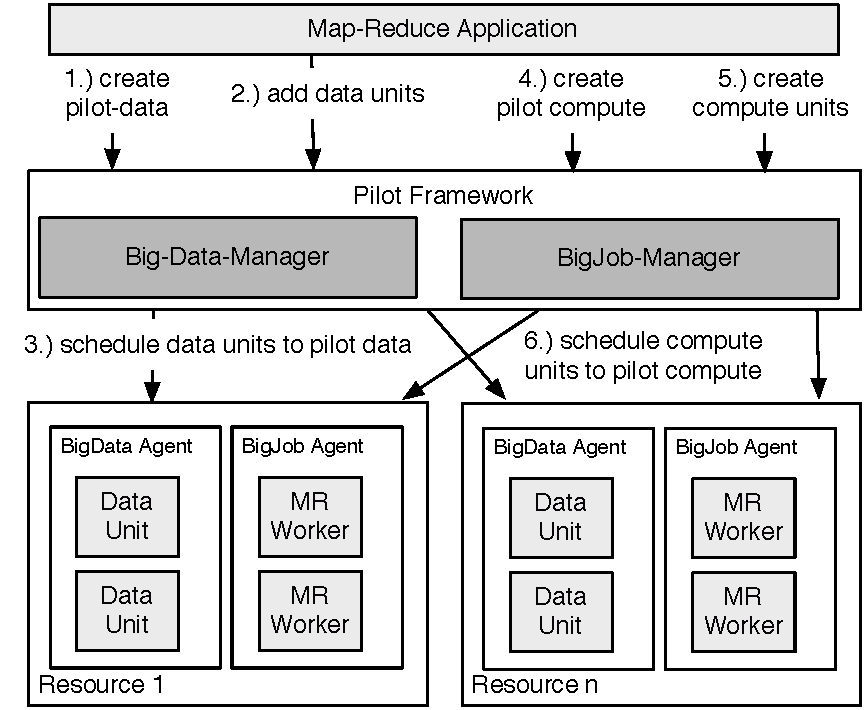
\includegraphics[width=0.4\textwidth]{figures/mapreduce-pilotdata.pdf}
	\caption{\textbf{Pilot-based MapReduce:} Each pilot (both compute and data 
	pilot) can be associated with an affinity label. The BigData and BigJob 
	Manager will ensure that CUs and DUs are placed with respect to these 
	requirements.}
	\label{fig:figures_mapreduce-pilotdata}
\end{figure}

The flow of a typical MapReduce application involves the chunking of the data,
the execution of the map compute tasks, shuffling and moving the intermediate
data to the reduce task and finally the execution of the for reduce tasks.
Pilot-MapReduce utilizes a set of compute and data pilots for this application
workflow:
\begin{enumerate}
	\item Initially, the MR manager allocates a set of compute and data 
	resources by starting a (or most often a set) of compute and data pilots 
	on different resources. In general, on each resource one compute 
	and one data pilot is co-located. The data pilot is either created with 
	reference to local input data or the input data is moved to the data pilot 
	after its creation. 

	\item \textbf{Chunking:} The input data is {\it chunked}. BigJob is used 
	as general abstraction for executing CUs. Thus, the MR-Manager executes a set of 
	chunk compute units via BJ. \label{stp:chunking}
	
	\item \textbf{Mapping:} The frameworks assigned a set of {\it map} CUs to 
	the chunks created in step~\ref{stp:chunking}. Again, BJ is used for managing the CUs. 
	BJ and BD ensures that CUs and DUs are co-located.
	
	\item \textbf{Shuffling:} \pnote{partitioning and sorting of 
        map output is part of map task}. \alnote{Hadoop Definitive Guide: ``The process by 
		which the system performs the sort and transfers the map outputs to the reducers as 
		inputs is known as the shuffle.'' - I would prefer to work with this definition 
		since it encapsulates this intermediate step very well. Rather then including it in 
		the mapping phase (even if it might be done partially by the mapper process.) }  
		After the processing is finished the output data is sorted and partitioned into 
		multiple DU. Then, data is moved from the map CUs to the location of the reduce 
		CUs. In a distributed 
		\pilotmapreduce with n reduces distributed evenly across m machines, n*(m-1) 
		parallel data transfers are initiated to complete the intermediate data movement. 
		\alnote{We need to introduce what we mean by a distributed PMR.}
	
	\item \textbf{Reducing:} The {\it reduce} tasks are prepared and 
	executed via BJ on the DUs representing the intermediate data. The 
	management of the data transfers is done by BJ and BD. For this purpose, 
	each reduce CU reference a certain DU as dependency.
	
	\item The \pilots are terminated.

\end{enumerate}

The Pilot-API provides a well-defined abstraction for supporting the
late-binding of compute and data units. The API also allows the expression and
management of relationships between data units and/or compute units. BigJob
and BigData provide an implementation of the Pilot-API. Both frameworks ensure
that the data and compute affinity requirements of the MapReduce applications
are met for each step of the MapReduce workflow.


\subsection{Pilot-MapReduce and Distributed Data}

An increasing amount of data that scientific applications need to operate on 
is distributed data. In many cases the place of data 
generation and processing are far apart: For example, the Earth Science Grid 
federates data of various climate simulations~\cite{ESG}. Meta-genomic 
workflows need to process and analyze data generated by various sequencing 
machines~\cite{Jha:2011fk}.

Several options for running Hadoop on distributed data have been
proposed~\cite{weissman-mr-11}: (i) in a global MapReduce setup one central
JobTracker and HDFS NameNode is used for managing a distributed set of
resources; (ii) in a distributed MapReduce setup multiple MapReduce clusters
are used: a MapReduce cluster close to the data source for pre-processing data
and a central cluster for aggregating the different de-central data sources.
The volume of the pre-processed data is generally lower and thus, can be
easily moved to another processing resource. Weissman
et.\,al~\cite{weissman-mr-11} show that a distributed setup leads in most
cases to a better performance than the utilization of a global Hadoop cluster.

A main drawback of this approach is the increased complexity: Hadoop is not 
designed with respect to a federation of multiple MapReduce cluster. Thus, 
setting up such a system requires a lot of manual efforts. \pilotmapreduce in 
contrast enables the MapReduce framework to reason about data and compute 
localities and is able to operate on a dynamic and distributed pool of storage 
and compute resources. BigJob and BigData will ensure that the affinity 
requirements of the MR framework are met.


\section{Experiments and Results}

In this section we analyze the performance and scalability of \pilotmapreduce
and compare/contrast it to Hadoop. For this purpose we run several experiments
on FutureGrid~\cite{fg}. We run the experiment on the FG resources: India, 
Sierra and Hotel. Each experiment is repeated at least three times.

For our Hadoop experiments, we use Hadoop 0.20.2. At the begin of each run a 
Hadoop cluster is started via the Torque resource management system on a
specified number of nodes. The first assigned node is used as master node
running the Hadoop JobTracker and the NameNode. \alnote{What further settings
did we use? max number map tasks etc?}. \pnote{The maximum number of maps or reduces that can run on a node is set to 1, so that the task can use entire node for running tasks and there wont be any memory problems with huge amounts of data. The shuffle phase is configured to start after map phase, since it is difficult to calculate individual phase times, as shuffle phase starts before map phase completes.}


\subsection{MapReduce-Based Applications}

MapReduce has been utilized in various science application. A key performance 
factor is the amount of data that must be moved through the MapReduce system. 
The degree of data aggregation of the map tasks is thus, an important 
characteristic of a MapReduce application~\cite{weissman-mr-11}.

In the following we investigate two application scenario: (i) WordCount, an
application with a high data aggregation and thus, a small volume of
intermediate data \pnote{ high aggregation means the output of both (map \& reduce phase) is much less than input, in wordcount the intermediate data is higher than input data, in our implementation it is 192 percentage of input data} and (ii) a Genome Sequencing application, with aggregation between High and zero data aggregation.\pnote { there is data aggregation, where the output is only 30 percentage of input data; but its not zero , or high aggreagation, its in between them... The main point I am trying to prove  is that distributed-PMR is better than Jon's DMR atleast in low aggregation applications like GS dpulicate read removal.
Why is that because, Pilot-data provides concurrent data transfers between machines and the dataunits- so ideal intermediate data transfer would be { max(time taken to transfer data related to a reduce} which is significantly less than entire output of 1st stage MR's of Jon's DMR configuration.}

\subsubsection*{Word Count}

The Word Count application is the basis for many machine learning use cases, 
used e.\,g.\ for the classification of documents or clustering. In general, 
the output of the mapping phase is significant smaller than the input.


\subsubsection*{Genome Sequencing}

High-throughput genome sequencing techniques provided by Next Generation
Sequencing (NGS) platforms are changing biological sciences and biomedical
research. The data volumes generated by sequencing machines is 
increasing rapidly. The processing of this data requires a sophisticated 
infrastructure. For this purpose, we utilize MapReduce to model an important 
part of the sequencing workflow: (i) the read alignment and (ii) the 
duplicate removal. The read alignment is implemented in the mapping phase of 
the application. The read outputs are filtered for duplicates in the reduce 
phase. For both steps, BWA~\cite{Li:2010:FAL:1741823.1741825} is used as tool. 
In contrast to Word Count, almost no aggregation of the input data occurs.

% \subsection{Measuring Job completion time}
Hadoop: Job completion time is measured as the MapReduce runtime in the main
cluster, which involves time taken for MapReduce map, shuffle and reduce
phases. To avoid overlap in calculating the map and shuffle phase times, we
configure Hadoop MapReduce to start shuffle phase after MapReduce map phase is
completed because with default configuration MapReduce shuffle phase might
start before map phase completes.\alnote{do we measure the time that it takes 
to setup the cluster? put data into hdfs?}

%%%%%%%%%%%%%%%%%%%%%%%%%%%%%%%%%%%%%%%%%%%%%%%%%%%%%%%%%%%%%%%%%%%%%%%%%%%%

\subsection{Characterizing Local-MapReduce: Word Count}

In the first experiment, we benchmark the performance of \pilotmapreduce and
Hadoop using a simple Word Count application on a single cluster varying resource
configurations. For both the mapreduces, 
a total of 8 nodes on India machine are used.  In all scenarios the input data is 
pre-staged on the respective resources, i.\,e.\ for Hadoop the data is located 
in the HDFS file system, for PMR the data is stored on a shared file system. 
We set the total number of reduces to 8 for both Hadoop and Pilot MapReduces; further, the default chunk size 
of 128\,MB is used.\alnote{HDFS \# replicas?} - \pnote{default 2}\alnote{how many reduces to we use for PMR?} \pnote{8}

On FutureGrid, we used 8 nodes for Hadoop and Pilot MapReduce on India cluster. 

% In case of Hadoop MR, data is already present on India cluster, but needs to be pushed into HDFS before Hadoop MapReduce is started. For local-PMR, data is already present on India cluster which is stored on a shared file system. For
% distributed-PMR, the total data is divided between India and Hotel cluster and
% is already present on shared file systems of each cluster. 


\pilotmapreduce: Job completion time is measured as the total runtime involved 
in chunking input data, MapReduce map, intermediate data transfer and reduce 
phases.

% \subsection{Evaluation}
We measured time-to-completion for each job. Figure~\ref{fig:figures_compMR} 
shows the results.

\begin{figure}[compMR]
	\centering
		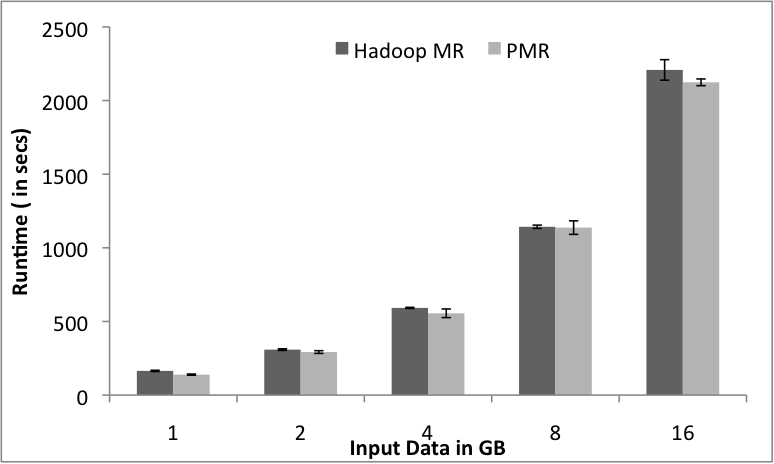
\includegraphics[width=0.47\textwidth]{figures/HMRvsL-PMRvsD-PMR.png}
	\caption{Pilot-MapReduce vs Hadoop MapReduce} \pnote{128MB; Yes i think it make sense to stick to local; why beacause
1. Local MR performs better than DMR when initial data transfer is considered.
2. If initial data transfer is considered, then Weismann's DMR should be considered to compare distributed-PMR, since we are using wordcount application, which has high aggregation.}
	\alnote{What is the chunk size? Distributed vs. non-distributed? }\pnote{Do we want to stick to local?}
	\alnote{How much data is moved from map to reduce phase?} \pnote{192.76 in case of wordcount} 
	\alnote{Do we have a distributed Hadoop setup as well?}\pnote{No}
	\alnote{Do we measure the time for putting the data into HDFS--Yes}
	\label{fig:figures_compMR}
\end{figure}

The time to solution increased linearly as data size increased for all cases. 
The map phase time of Hadoop is 11.6\,sec.

% greater than Map phase time of Local-PMR because Hadoop MR involves preparing input splits and starting the map tasks, whereas in Pilot MapReduce, chunk time is considered seperatly and Map phase involves submitting of map compute units. The chunking time of distributed-Pilot MapReduce is less when compared to Local-PMR, since the data is halved and distributed to two machines. \pnote{ Andre::question::Hadoop uses logical splitting of files, where as PMR chunks the files physically, wiritng to disk, this is a performance bottlneck. Is acessing a single file, by many parallel subjobs cause problems?}. The shuffle phase is considered only in Hadoop MapReduce, where as the exchange is involved in Pilot MapReduce. The input to the reduce phase in all the three MapReduce increased linearly with input data. In local-PMR is < 1sec as the data is moved within cluster using SAGA file adaptor. In distributed PMR, the time to exchange data between India and Hotel also increased linearly with input data size. The Reduce phase is high for Pilot MR since the reduce compute units has to read intermediate data from the disk and write output data to the disk, where as in Hadoop MapReduce reduce phase, the intermediate data is available in memory and write the output to HDFS.


\begin{figure}[compMR_16GB]
	\centering
		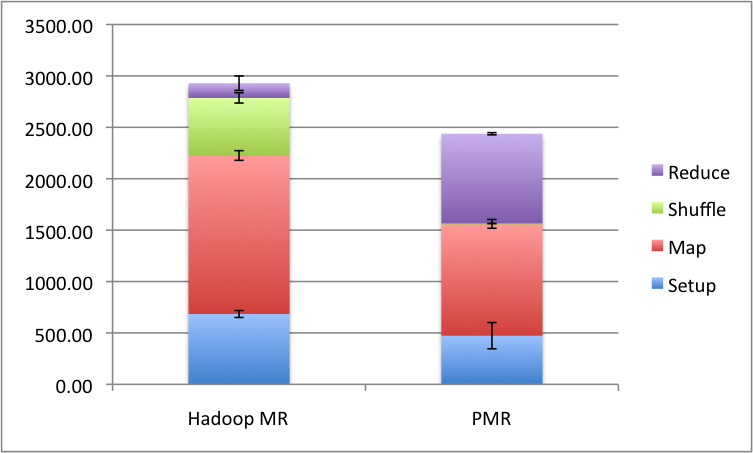
\includegraphics[width=0.47\textwidth]{figures/comparision_16gb.png}
	\caption{Wordcount on 16GB plain-text data with 8 workers, 8 reduces and 128MB chunk size on India.}
	\alnote{Do we have some larger volumes of data? In our old MR paper we
	had 10 GB of data.} \pnote{16GB data is added}
	\alnote{Time to put data into HDFS?} \pnote{ included in the graph?}
	\alnote{Can we have a stacked bar chart?}
	\alnote{Why are our reduces so slow?} \pnote{ Hadoop reduce tasks read intermediate data either from memory or hdfs; whereas In pilotMR- the reduces read/write  to a shared file system}
	\label{fig:figures_compMR_16GB}
\end{figure}


Observed performance issues:
1) HDFS performs better when nodes local data directory is used.. But performance degrades if shared storage is used. 			
2) when a single node is used to launch all workers, hadoop fails with lot of memory problems, whereas PMR successfully completed all tasks.			
reasons for this problem

http://tech.backtype.com/the-dark-side-of-hadoop+J204		

compute node memory statistics.

(python)-bash-3.2$ hostname
i69
(python)-bash-3.2$ free -m
                  total          used       free     shared    buffers     cached
Mem:         24081       4524      19557          0        146       4128
-/+ buffers/cache:       248      23832
Swap:         2047          0       2047
	

         - varying input size (1GB, 2GB, 4GB, 8GB - experiments repeated for 3 times atleast..)

%\subsubsection*{Distributed MapReduce: Word Count} 



\subsection{Characterizing: Genome Sequencing}


\begin{figure}
 \centering
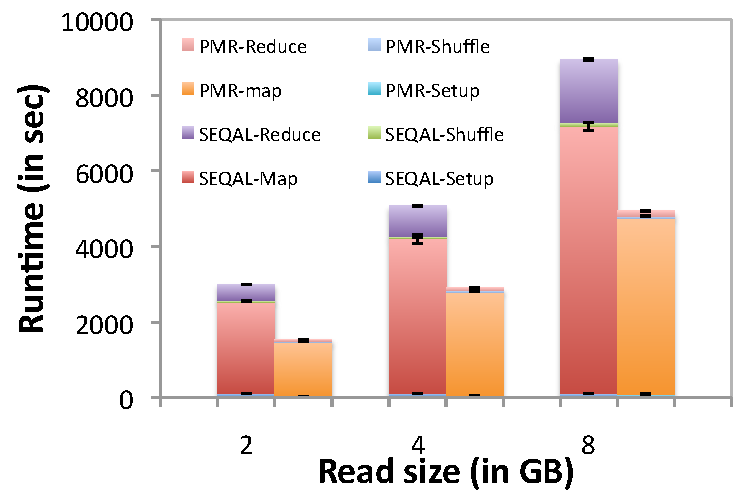
\includegraphics[scale=0.50]{figures/seqalvslocalpmr.pdf}
\caption{\small Hadoop-based SEQAL vs. Pilot-MapReduce:  BWA is the aligner for the map phase; number of nodes=4; number of workers/node=2, number of reducers=8, number of reads/chunk=292763 for PMR ==128MB for hadoop based apps
\alnote{Can we adjust the style and include the map/shuffle/reduce time in a stacked bar chart?}}
 \label{fig:comp_with_seqal_1} 
\end{figure}

\begin{figure} 
 \centering
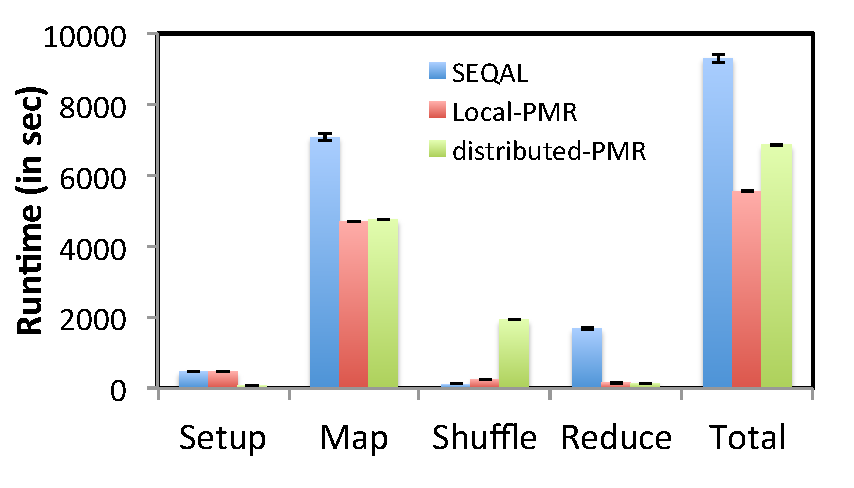
\includegraphics[scale=0.50]{figures/8GB_phasewisetimes.pdf}
\caption{\small Comparison between SEQAL and Pilot-MapReduce.  The runtime contributions from each step are compared in details. BWA is the aligner for the map phase; ********DMR provides scale-across********** as two machines sierra and hotel are used.}
  \label{fig:comp_with_seqal_2} 
\end{figure}



2. Distributed PMR vs Weissmann's implementation of  DMR

\begin{figure}[jonsdmr]
	\centering
		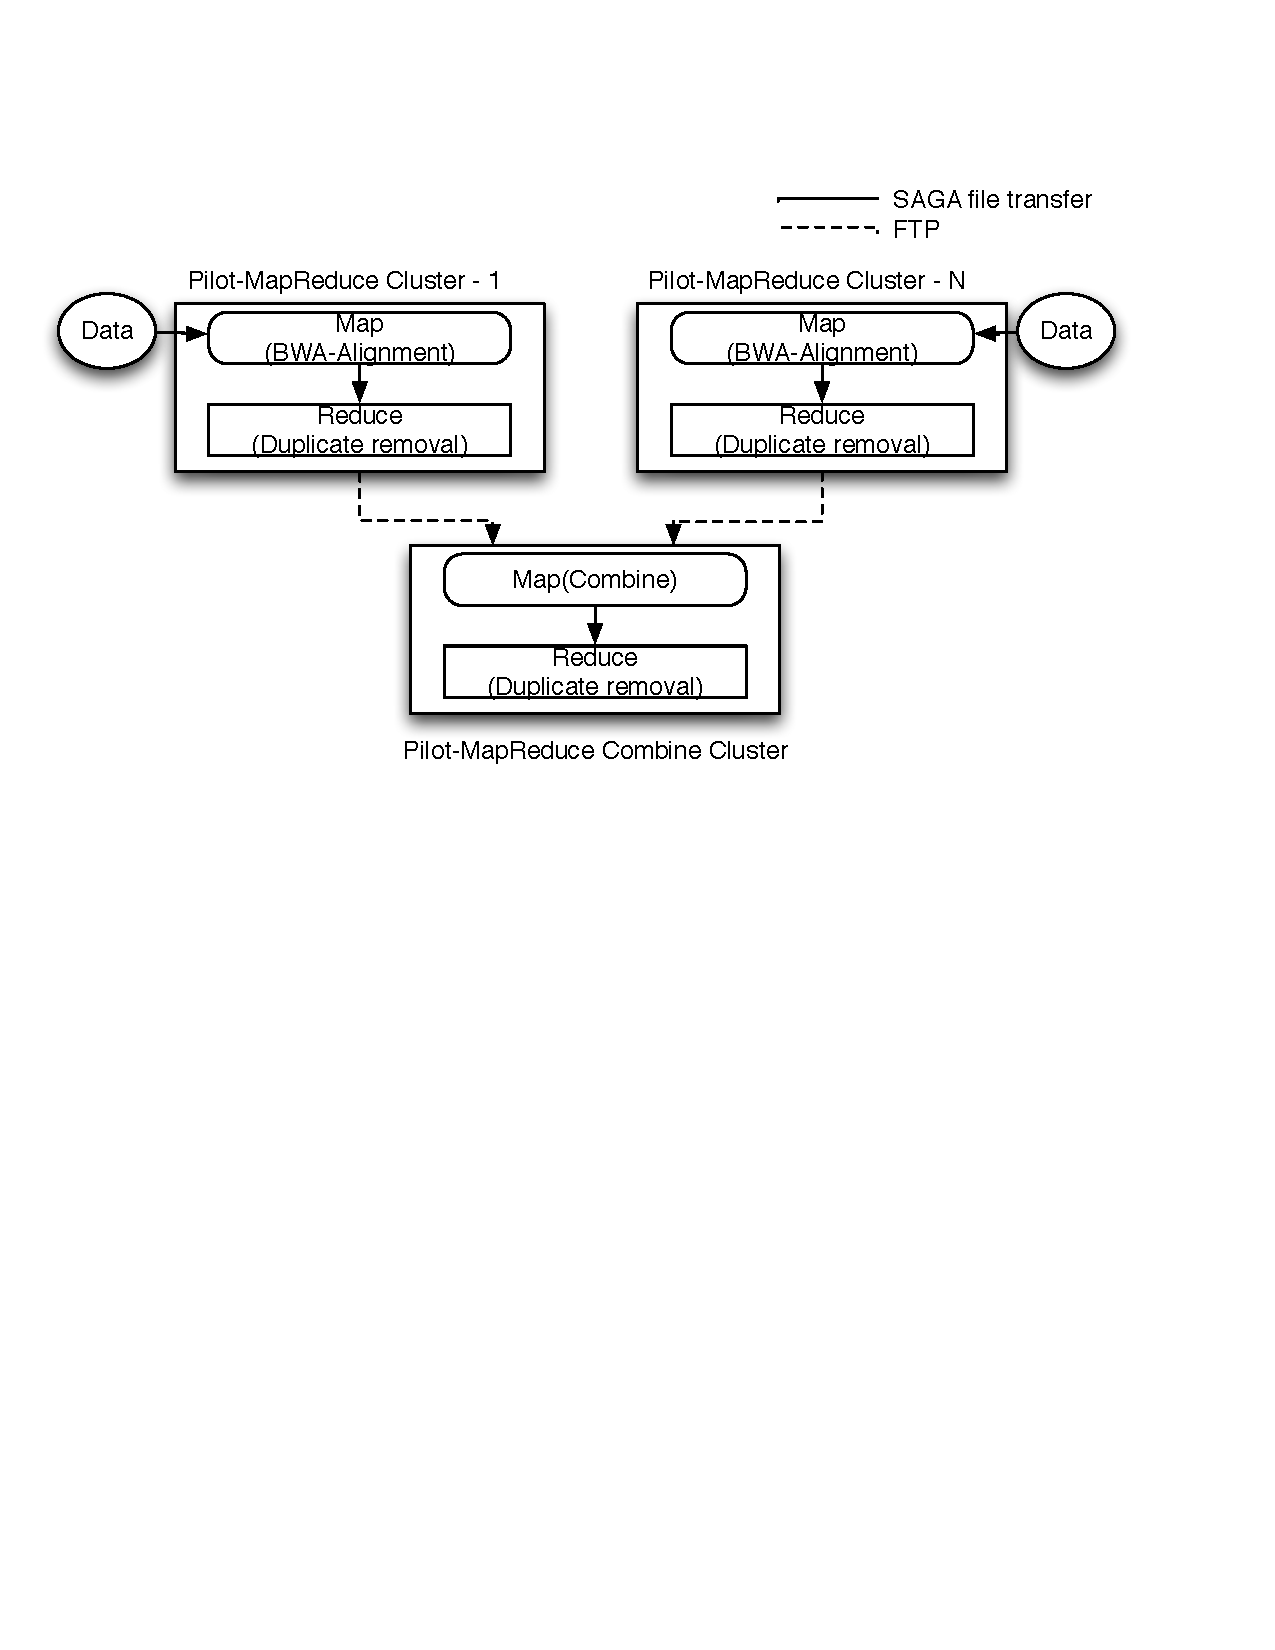
\includegraphics[width=0.47\textwidth]{figures/jon_dmr_dup_rm_app.pdf}
	\caption{Weissmann's dmr for GS application} 
	\label{fig:figures_jonsdmr}
\end{figure}

In this experimentation section, we try to compare the distributed PMR implemenation with \cite{weissmann} DMR implemenation using genome sequencing application which has low aggreagation workload. The DMR is configured using 3 local Pilot-MapReduces. The number of workers on each cluster is set to 32 , chunk size to 625k sequences and number of reduces to 8 in both PMR and DMR. We conduct the experiments on India and Hotel futuregrid machines. The job completion time for DMR is max time of both individual MapReduce jobs on India and Hotel, plus the result combination step to combine the sub-results into the final result at a single data lcoation on Hotel.  We considered Hotel machine to combine the sub-results to optimize the data transfer, which is in case of using another machine. We choosed Hotel instead of India, because Hotel is faster than India machine.


\pnote{Weissmanns paper doesn't talk about low workload scheme applications where reduce output is still significantly large.. ( it talks about zero, high, balooning ).. so we have a model for these type of applications. why weissmanns DMR is choosed?? LMR involves huge amount of initial data transfer. GMR need global filesystem across clusters, which is difficult to have, and latencies issues in moving files. So, DMR is a potential choice over LMR and GMR. }

In ~\cite{weissman-mr-11}, different workload data aggregation schemes are evaluated.  
High Aggregation: The MapReduce output is multiple orders of magnitude smaller than the input, e.g. Wordcount on English plain-text.
Zero Aggregation: The MapReduce output is the same size as the input, e.g. the Sort workload.
There is no MapReduce configuration regarding low aggregation schemes, where the output data is significant and between high and zero aggregation schemes. In this experiment, we try  to prove that \pilotmapreduce is a best model for low aggregation schema applications. We choose ~\cite{weissman-mr-11} DMR configuration and compare it with \pilotmapreduce with genome sequence application, which produces significant amount of output and neither high aggreation nor zero aggregation. We ran experiments with 20GB, 40GB and 80GB on two machines and 30GB, 60GB , 120GB on 3 machines.

\begin{figure}[dmrvspmr]
	\centering
		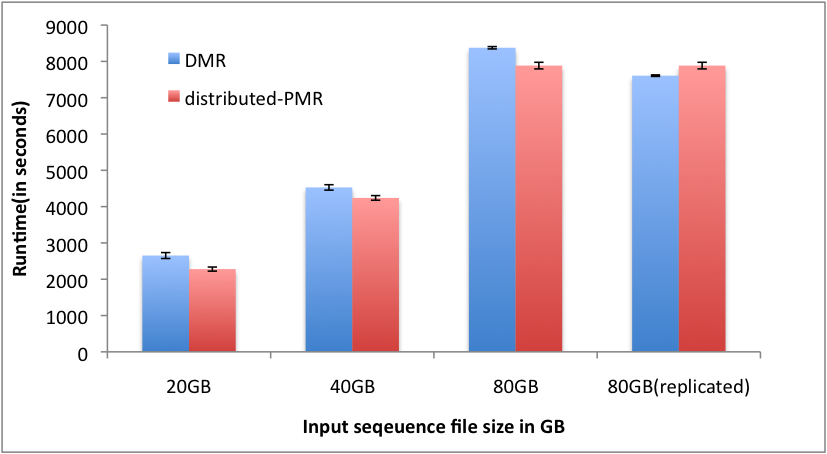
\includegraphics[width=0.47\textwidth]{figures/dmrvspmr.png}
	\caption{DMR vs PMR using Duplicate read removal application on 2 machines} 
	\label{fig:figures_dmrvspmr}
\end{figure}

A correlation exists between the input sequence sizes and performance of MapReduce configurations. As the data size increases, the runtime for both the frameworks increases. 
In PMR, the increase in runtime is due to the amount of data, to be processed by map phase , moved in the shuffle phase  and processed by reduce phase. In DMR, the increase in runtime is due to increase in data to be processed by map and reduce phases and the amount of data to be moved to the second level of MapReduce.

For 20GB, 40GB and 80GB PMR performs better than DMR, because the effective amount of data to be transferred is less than the amount of data to be transferred in DMR.
The performance of PMR decreases 





DMR outperforms PMR if pilot-data doesn't transfer intermediate data concurrently. At the same time, if the concurrency  is not tuned properly, it might cause bandwidth problems.


PMR tts = max( map  on india, map on  sierrra, map on hotel) + max( exchange of intermediate data between all machines(n) ( r * n-1 concurrent exchanges)) + max ( reduce phase on  india, reduce on  sierrra, reduce on hotel)

--- experiments done for local PMR on each individual cluster.. once time taken to trasnfer intermediate data between machines is obtained.. then tts for PMR can be caluculated and compared to DMR.




\section{Conclusions and Future Work}


Extending BigData: Access data through BigData abstraction.

BigData \& Realtime

Higher-level abstraction for MapReduce: Hive, Pig


Contrast to Hadoop:
Pilot-MapReduce provides more flexibility and building block, e.g. flexible 
usage of sorting, more fine-grained control of data transfers etc.

%
% The following two commands are all you need in the
% initial runs of your .tex file to
% produce the bibliography for the citations in your paper.
\bibliographystyle{abbrv}
%\bibliographystyle{unsrt}
\bibliography{pilotjob,saga,saga-related,mrbib}  % sigproc.bib is the name of the Bibliography in this case
% You must have a proper ".bib" file
%  and remember to run:
% latex bibtex latex latex
% to resolve all references
%
% ACM needs 'a single self-contained file'!
%


cite moore's law
cite script used to convert fastq to qseq
cite reference paper used to implement duplicate removal application.


\subsection*{Acknowledgments}
\scriptsize
This work is funded by NSF CHE-1125332 (Cyber-enabled Discovery and
Innovation), HPCOPS NSF-OCI 0710874 award, NSF-ExTENCI (OCI-1007115) and NIH
Grant Number P20RR016456 from the NIH National Center For Re- search
Resources. Important funding for SAGA has been provided by the UK EPSRC grant
number GR/D0766171/1 (via OMII-UK) and the Cybertools project (PI Jha) 
NS-F/LEQSF (2007-10)-CyberRII-01. SJ acknowledges the e-Science Institute,
Edinburgh for supporting the research theme. Distributed Programming
Abstractions \& 3DPAS. SJ ac- knowledges useful related discussions with Jon
Weissman (Minnesota) and Dan Katz (Chicago). We thank J Kim (CCT) for
assistance with genome sequencing application. This work has also been made
possible thanks to computer resources provided by TeraGrid TRAC award
TG-MCB090174 (Jha) and BiG Grid. This document was developed with support from
the US NSF under Grant No. 0910812 to Indiana University for FutureGrid: An
Experimental, High-Performance Grid Test-bed.

\end{document}
